%----------------------------------------------------------------------------------------
%PACKAGES AND OTHER DOCUMENT CONFIGURATIONS
%----------------------------------------------------------------------------------------

\documentclass[11pt]{article} 

\usepackage[top=.4in, bottom=1in, left=1in,
right=.3in]{geometry} 

\geometry{a4paper} 

\usepackage{graphicx}

\usepackage{float} 

\usepackage{wrapfig}

\linespread{1} % Line spacing

\usepackage{ragged2e}

\usepackage{enumitem}


%\setlength\parindent{0pt} % Uncomment to remove all indentation from
%paragraphs
\graphicspath{{../../pics/}} 


\begin{document}

\begin{center} \huge{\bfseries{Hierarchical goal abstraction for sensorimotor
    agency}}\\ {The model -- Draft 0.1 \today}\\[3cm] \end{center}


\begin{figure}[H] \centering \includegraphics[width=.8\textwidth]{schema_simpl}
    \caption{Architecture of the model.} \label{fig:blueprint} \end{figure}

\section{The model}
\label{sec:model}

\subsection{The task}
\label{sec:task}

These simulations are a simplified version of the buzzer
experiments. We use a simple 2-dimensional agent composed of
2 arms (2 segments with 3 joints each), and a torso
connecting them. On the whole body of the agent are
positioned N touch sensors, activated when reached by one of
the two edges of the arms (the ``hands'').

Simulations are divided in two phases, each composed of X
trials. A trial ends if a determined amount of time is
reached or if a match event (see sec.~\ref{sec:definitions}) occurs. 

On the first phase, the agent starts exploring its body space
with random movements. When a sensor is activated, the
system starts learning the proper posture (end-point) needed
to determine that activation. In particular, the learning
process is driven by competence-based intrinsic motivations
(CB-IMs), so that the system continues to focus on that
particular posture as long as it is improving its ability to
achieve it. The activations of the touch sensors trigger the formation of
internal abstractions together with the movements (end-point
postures) necessary to determine those activations.

In the second phase, a token is put on one of the sensors of the
agent (to simulate the buzzer touching that part of the
body). On the basis of previosly acquired skills, the agent
has to learn to reach for the token on its body.

\subsection{Expected behaviour}
\label{sec:behaviour}

In the first phase, we expect the system to explore its body
space and its actions creating a complete sensory-motor
abstraction map.  We also expect that the more the system is
getting close to complete the map, the slower become the
learning process: when the agent has learnt to reach all the
different part of its body it has formed a sensory-motor map
that is no more modified during the first phase of the
experiment.

In the second phase, we expect the system to exploit the
autonomously acquired knowledge/competence to reach the place where
the token/buzzer is positioned. 

\section{Definition of key terms}
\label{sec:definitions}

\begin{itemize}[leftmargin=3cm]  
    \item[\textbf{goal:}]

        \begin{itemize}

            \item A state of the world (a particular disposition of the touch sensors, in this version) that the \textbf{goal-abstraction layer}
                can identify and distinguish from others
                (section~\ref{sec:abstraction}).

            \item A configuration of the \textbf{action-selection layer} that
                can be linked to a proper action (section~\ref{sec:selection}).

        \end{itemize}

\end{itemize}

\begin{quote}
    \texttt{
        Note: the goal-abstraction layer has the same dimensionality of\\ 
        the goal-selection layer so that they can be compared.
    }

\end{quote}

\begin{itemize}[leftmargin=3cm]  

    \item[\textbf{match:}]

        \begin{itemize}

            \item The occurrence of an identical configuration of the
                goal-abstraction and goal-selection layers. 

        \end{itemize}    

    \item[\textbf{prediction:}]

        \begin{itemize}

            \item Computation of the probability that given a configuration of
                the goal-selection layer the agent will be able to obtain a state in which
                the goal-abstraction layer has the same configuration
                (\emph{match} event). 

        \end{itemize}  

    \item[\textbf{error:}]

        \begin{itemize}

            \item Difference between the prediction and the real occurrence of
                a \emph{match} event within a trial.

        \end{itemize}  

\end{itemize} 

\section{Simulator}
\label{sec:simulator}

\begin{itemize}

    \item \textbf{Environment:} the simulation takes place
        in a 2-dimensional space without physics.

    \item \textbf{Agent:} \begin{itemize}

            \item The body of the agent is composed of the 2
                arms plus a segment joining their origins

            \item Each arm has 3 joints (3DoF)

            \item N touch sensors all over the body.

        \end{itemize}

    \item \textbf{Agent sensory information}
    	
    In this first version of the model, the system only
    receives information from the touch sensors. In the
    final version visual information and proprioception will
    be added to the sensory input of the system.

        \begin{itemize}

            %\item \texttt{vision (V):} a 20x20pixels retina on which the body
                %(black line on figure~\ref{fig:blueprint}) is depicted in the
                %current position.

            %\item \texttt{proprioception (P):} a 20x20pixels retina on which
                %the current angles of joints are represented.

                %Encoding:

                %\begin{itemize} 

                    %\item Angles are encoded as 2D gaussians on a horizontal
                        %line centered in the middle of the retina. 

                    %\item The position of each gaussian on the horizontal line
                        %is related to the position of the related joint in the
                        %one-dimentional space of the body.

                    %\item The variance of each gaussian on the y-axis is
%                        related to the amplitude of the represented joint
%                        angle.

                    %\item The variance of each gaussian on the x-axis is a
%                        proportion of the one on the y-axis, so that
%                        overlapping between gaussians is not too much.
%
%                \end{itemize} 

            \item \texttt{input from the touch sensors (T):}
                a 20x20 pixels retina on which the current
                activations of the N touch sensors are
                represented.

%                Encoding:
%
%                \begin{itemize} 
%
%                    \item Sensors are encoded as 2D gaussians on a horizontal
%                        line centered in the middle of the retina. 
%
%                    \item The position of each gaussian on the horizontal line
%                        is related to the position of the sensor in the
%                        one-dimentional space of the body.
%
%                    \item The variance of each gaussian on the y-axis is
%                        related to the amplitude of the activation of the
%                        represented sensor.
%
%                    \item The variance of each gaussian on the x-axis is a
%                        proportion of the one on the y-axis, so that gaussians
%                        do not overlap too much.
%
%                \end{itemize} 

        \end{itemize}

\end{itemize}



\section{Controller} 
\label{sec:controller}

The controller takes the sensory information at each time
step and produces a motor command, consisting in the
requested position of the 6 joint angles (3 for each arm).

More precisely, the actual motor command is a composition
between the output of the controller and a noise signal. The
more the system learn its skills, the more the actual motor
command rely only on the output of the controller (see 
sec.~\ref{sec:actiontriggering} for more details).

\subsection{Abstraction}
\label{sec:abstraction}

The sensory information provided at each time step is
further processed by computing the finite difference with
the information given at the previous time step. As a
result, the input is composed by a retina containing the
\emph{derivative} of the (T) described above.

The result of this processing is sent as input to a
self-organizing map (SOM).  The output of the SOM is further
processed so that all output units have 0 activation except
the one whose weights are the closest to the current input,
which has 1 activation.  

This process generates high-level abstractions of the
sensory input that can be compared with the abstractions of
the end-point postures. In this way a sensory-motor map can
be acquired.

The learning of the SOM is also modulated by the activity of
the goal-prediction layer (see sec.~\ref{prediction})

%
%\begin{figure}[H]
%    \centering
%    A 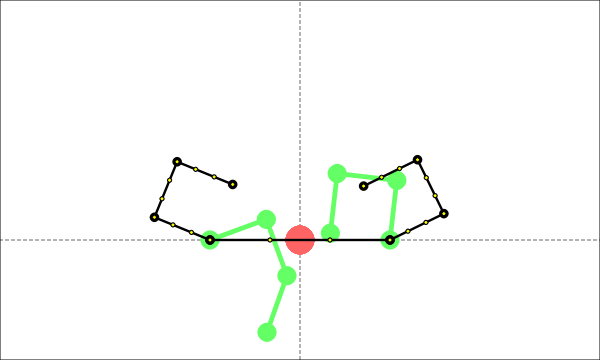
\includegraphics[width=.6\textwidth]{SOMs_kinematics}\\
%    B 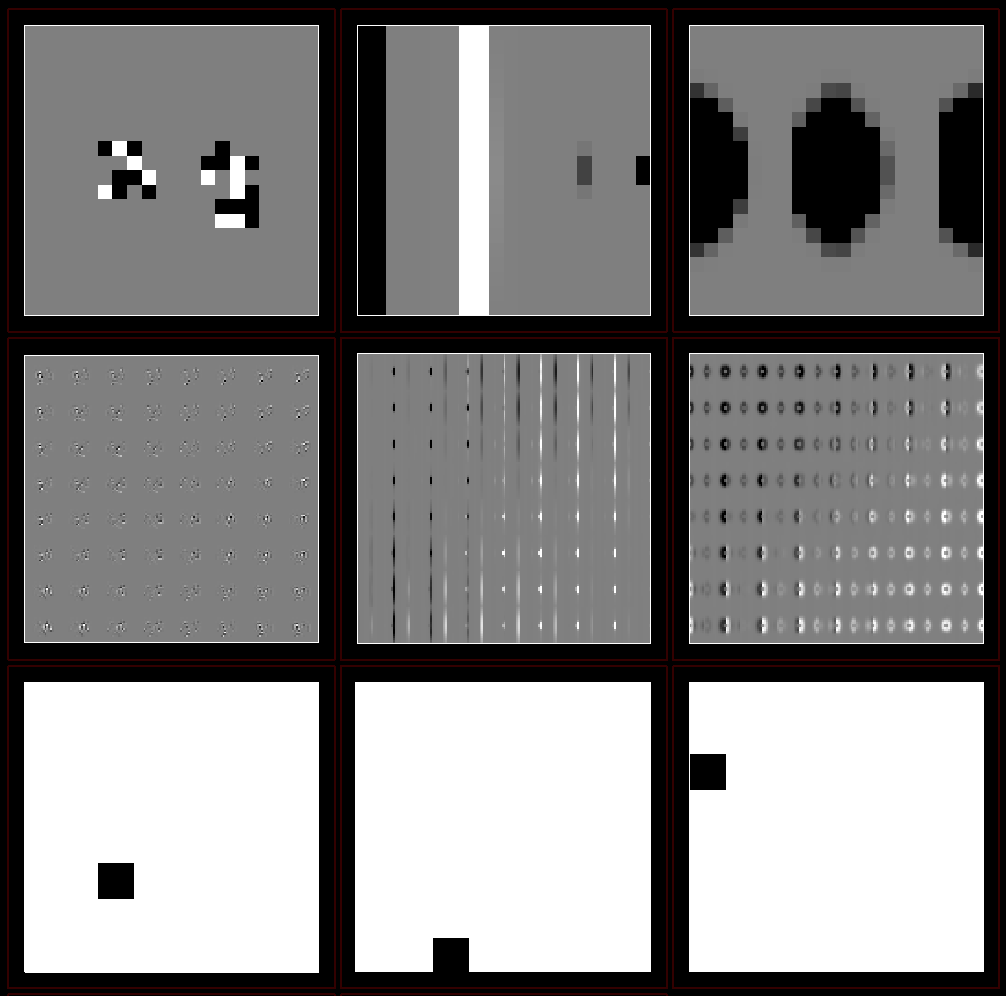
\includegraphics[width=.6\textwidth]{SOMs}
%
%    \caption{
%        Activity of the 1st layer of the hierarchical network. A) The
%        current position of the agent. B) The first row shows the derivatives of
%        the (V),(P) and (T) retinas. The second row show the current status of the 
%        weights of the SOMs. Each of the three plots shows a 8x8 matrix of 
%        20x20 retinas. Each 20x20 retina represents the weights connecting 
%        the input retina to an output unit. The third row shows the output layers
%        of each SOM. the black pixel represents the winner unit for the current input.
%    }
%
%    \label{fig:soms}
%\end{figure}
%
%The 2nd layer of the hierarchical network is composed of two SOMs. The 1st SOM in
%the 2nd layer merges the 16x8pixel output coming from the (V) and the (P) SOMs
%in the first layer into a 4x4pixel output. The 2st SOM in the 2nd layer merges
%the 16x8pixel output coming from the (P) and the (T) SOMs in the first layer
%into a further 4x4pixel output. The 3rd layer is composed by a single SOM
%mergng the outputs of the 2nd layers (a 8x4pixels retina) into a 4x4pixels
%output. The 4rd layer gets all the outputs from the previous layers as a
%(3*400+2*32+16)pixels flatten input vector and merges it into a 3x3pixels
%output. \textbf{The 4th layer gives abstracted representations of the 3-modal
%    sensory information as 9 identifiable states.  }

\subsection{Goal selection}
\label{sec:selection}

The goal-selection layer is a matrix of units with the same
numerosity of the abstraction layer. At the beginning of
each trial one of the goal-units is selected. The
probability for each unit to be selected depends on its
value (plus noise), determined by the running averages of
the prediction error related to that goal (see
section~\ref{sec:prediction}). Each average is updated at
the end of the trials in which the corresponding unit is
actually selected: as a result, these running averages
convey information about the current amount of error
related to each goal-unit. 

While the agent is learning, each unit is associated with
the production of one particular end-point posture. 

\subsection{Goal prediction}
\label{sec:prediction}

The \textbf{goal-prediction layer} takes the activation of
the goal-selection layer as input and return a
\textbf{prediction of a \emph{match} event} (i.e. a
prediction of the achievement of the selected goal). This
prediction is compared with the actual occurrence of a
\emph{match} event at the end of each trial.
The result of this comparison (the \emph{error}) is used
both to update the parameters of the goal-prediction layer
and to determine the activation of the corresponding unit in
the goal-selection layer (see section
\ref{sec:selection}).

Moreover, the activity of the goal-prediction layer is used
to modulate the learning of the abstraction layer and of the
motor controller.


\subsection{Action triggering}
\label{sec:actiontriggering}

The \textbf{motor output} of the controller is represented
by the activation of 6 readout units of an echo-state
network (ESN, see the appendix). Each readout unit gives
the current amplitude of a joint angle of the 2-arm agent.

The input to the ESN is provided by the goal-selection layer. The activation of
the goal-selection layer is connected to the ESN in two ways: 

\begin{enumerate}

    \item It steadily excites distinct subpopulations of the ESN
        reservoir based on the current selection during a trial. This
        excitation triggers the proper dynamics of the reservoir and
        guaranties that the reservoir activity fades to a distinct fixed
        point depending on the selection.

    \item It inhibits distinct subpopulations of the ESN reservoir based on
        the current selection. This inhibition allows to select different
        dynamics in the network.

\end{enumerate}

The weights connecting the reservoir to the readout units of the ESN are
updated via a reward-based online learning rule, with \textbf{the \emph{match}
event triggering the reward signal.} Also this learning
process is modulated by the activity of the goal-prediction
layer (i.e. on the basis of intrisic motivations)\\

The actual motor output is composed of the activation of the
6 readout units plus some \textbf{exploratory noise} noise
(6 sinusoidal oscillators whose parameters are set randomly
at each trial). The amplitude of the noise depends on the
amount of previous \emph{match} events given the same goal
selection.  As soon as matches become frequent the motor
output becomes completely dependent on the activity of the
readout units (\textbf{exploitation} with no noise). 


\section{Appendix: the Echo-State Network}
%
\begin{figure}[H] 
 
    \centering 

    A 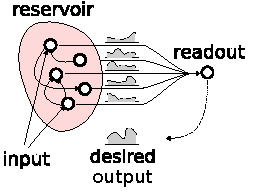
\includegraphics[width=.6\textwidth]{reservoir} 
    
    B 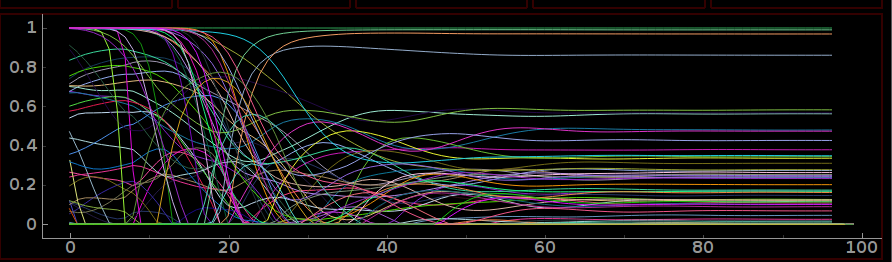
\includegraphics[width=.6\textwidth]{ESN} 

    \caption{ The echo-state network.  }
    
    \label{fig:esn}

\end{figure}

Figure~\ref{fig:esn} shows a general schema of the
functioning of an ESN. inputs reach sparsely the internal
units of the reservoir. 

Internal units are connected with each other via sparse
random connections. Learning consists in the update of the
external weights connecting the reservoir to one or more
readout units. After learning, the readout units reproduce a
learnt trajectory in relation to a specific input. 

Figure~\ref{fig:esn}B shows the typical activation of the
reservoir in the model. During the second half of the trial
the ESN reaches a fixed point that is peculiar of for the
current input (a selected goal).

%


\end{document}



